\subsection{Dati e risultati}

\paragraph{Flip-Flop SR}

Il flip-flop SR (Set-Reset, il nome deriva dalle terminazioni) è il primo elemento
di memoria che incontriamo in questo corso. È un circuito sequenziale e non
combinatorio, nel senso che il suo output dipende da quello che è avvenuto prima
e non dallo stato delle entrate.

\begin{figure}[b]
	\centering
	\begin{circuitikz}
		\draw
			(2, 0) node[nand port] (s) {}
			(2, 3) node[nand port] (r) {}
			(5, 0) node[nand port] (q) {} (4.75, -0.75) node {$U_1$}
			(5, 3) node[nand port] (qbar) {} (4.75, 3.75) node {$U_2$}
			(0, 0) node[left] {S} -| (s.in 1) -| (s.in 2)
			(0, 3) node[left] {R} -| (r.in 1) -| (r.in 2)
			(s.out) -| (q.in 2)
			(r.out) -| (qbar.in 1)
			(q.out) --++ (0.5, 0) node[right] {Q} --++ (0, 0.5) 
			(qbar.out) --++ (0.5, 0) node[right] {$\bar{\text{Q}}$} --++ (0, -0.5)
			(qbar.in 2) --++ (0, -0.5) -- (5.65, 0.5)
			(q.in 1) --++(0, 0.5) -- (5.65, 2.5)
		;
	\end{circuitikz}
	\caption{}
	\label{fig:ff_sr11}
\end{figure}

Il flip-flop SR è riportato in figura \ref{fig:ff_sr11}. Questo piccolo e straordinario circuito
si basa sulla dipendenza reciproca tra entrate ed uscite delle porte NAND $U_1$ e $U_2$.
Non è difficile capire, provando a immaginare il funzionamento del circuito per ciascuna
combinazione di input S e R, che la tabella di verità del circuito è la tabella \ref{tab:ff_sr11}

\begin{table}
    \centering
    \begin{tabular}{llll|ll}
	    \toprule
		    S & R & $\overline{S}$ & $\overline{R}$ & Q & $\overline{Q}$ \\
	    \midrule
		    0 & 0 & 1 & 1 & x & $\overline{x}$ \\
		    0 & 1 & 1 & 0 & 0 & 1 \\
		    1 & 0 & 0 & 1 & 1 & 0 \\
		    1 & 1 & 0 & 0 & 1 & 1 \\
	    \bottomrule
	\end{tabular}
    \caption{Tabella di verità del circuito in figura \ref{fig:ff_sr11}. S ed R sono gli ingressi, mentre Q e $\overline{Q}$.}
    \label{tab:ff_sr11}
\end{table}

L'aspetto notevole è il fatto che quando R e S sono entrambi a 0, l'output rimane
uguale a quello che è stato impostato in precedenza. In pratica il circuito mantiene in memoria
un informazione. Questo è possibile poiché un ingresso di ciascuna delle porte NAND $U_1$ e $U_2$
rimangono a 0, facendo passare l'informazione contenuta all'uscita dell'altra porta (negata).
Il sistema è quindi stabile. Per impostare il valore delle uscite si possono utilizzare
le configurazione $S=1$ e $R=0$ oppure $S=0$ e $R=1$. Il caso R e S entrambi a 1 è invece da
evitare, perché porta il circuito in uno stato non ben definito. Infatti una volta che gli ingressi
cambiano da 1 a 0 non si sa più qual'è l'output, perché esso dipende da come avviene la transizione (da quale passa prima a 0).

Questo piccolo circuito è quindi un elemento di memoria che può immagazzinare un dato binario.
Non ci è rimasto che verificare il funzionamento del circuito utilizzando la schedina con i LED,
test che ha dato esiti positivi. 

\paragraph{Flip-Flop SR sincronizzato}

Il flip-flop (FF) che abbiamo costruito nel precedente paragrafo viene detto asincrono poiché
cambia stato quando l'input cambia. Vogliamo ora costruire un FF sincrono. In un flip-flop
sincrono l'output cambia stato al comando di una cosiddetta linea di clock (CLK).

\begin{figure}
	\centering
	\begin{circuitikz}
		\draw
			(2, 0) node[nand port] (s) {}
			(2, 3) node[nand port] (r) {}
			(5, 0) node[nand port] (q) {} (4.75, -0.75) node {$U_1$}
			(5, 3) node[nand port] (qbar) {} (4.75, 3.75) node {$U_2$}
			(0, 0) node[left] {S} -| (s.in 2)
			(0, 3) node[left] {R} -| (r.in 1)
			(s.out) -| (q.in 2)
			(r.out) -| (qbar.in 1)
			(q.out) --++ (0.5, 0) node[right] {Q} --++ (0, 0.5) 
			(qbar.out) --++ (0.5, 0) node[right] {$\bar{\text{Q}}$} --++ (0, -0.5)
			(qbar.in 2) --++ (0, -0.5) -- (5.65, 0.5)
			(q.in 1) --++(0, 0.5) -- (5.65, 2.5)
			(0, 1.5) node[left] (clk) {CLK} -| (r.in 2)
			(clk) -| (s.in 1)
		;
	\end{circuitikz}
	\caption{}
	\label{fig:ff_sr_sync11}
\end{figure}

La figura \ref{fig:ff_sr_sync11} mostra un FF sincrono. Il dato viene scritto nella memoria
soltanto quando il clock è a 1. Nella modalità $CLK=0$ il flip-flop rimane nello stato in cui è stato impostato.
Infatti quando uno degli ingressi delle porte NAND è nullo, il suo output è certamente 1, quindi
agli ingressi di $U_1$ e $U_2$ ci sono degli 1 logici. Ci troviamo quindi nella configurazione
che mantiene il dato in memoria.

Anche in questo caso la verifica è stata immediata.

\paragraph{Flip-Flop RS D-type}

È spesso utile poter salvare lo stato di un segnale. Torna utile per questo scopo il flip-flop
di tipo D. Il circuito è riportato in figura \ref{fig:ff_sr_dtype11}. Non c'è molto
da commentare sul circuito poiché è molto simile ai precedenti. La differenza è che
quando il CLK è alto viene immagazzinato in Q il segnale proveniente dall'ingresso D.

\begin{figure}
	\centering
	\begin{circuitikz}[transform shape, scale=0.95]
		\draw
			(2, 0) node[nand port] (s) {}
			(2, 3) node[nand port] (r) {}
			(5, 0) node[nand port] (q) {}
			(5, 3) node[nand port] (qbar) {}
			(-0.75, 3) node[not port] (not) {}
			(-2, 0) node[left] (d) {D} -| (s.in 2)
			(d) -| (not.in)
			(not.out) -- (r.in 1)
			(s.out) -| (q.in 2)
			(r.out) -| (qbar.in 1)
			(q.out) --++ (0.5, 0) node[right] {Q} --++ (0, 0.5) 
			(qbar.out) --++ (0.5, 0) node[right] {$\bar{\text{Q}}$} --++ (0, -0.5)
			(qbar.in 2) --++ (0, -0.5) -- (5.65, 0.5)
			(q.in 1) --++(0, 0.5) -- (5.65, 2.5)
			(0, 1.5) node[left] (clk) {CLK} -| (r.in 2)
			(clk) -| (s.in 1)
		;
	\end{circuitikz}
	\caption{}
	\label{fig:ff_sr_dtype11}
\end{figure}

\begin{figure}
	\centering
	\begin{circuitikz}
		\draw
			(0, 1.5) node[rground] (gnd) {}
			(1, 1.5) node[spdt] (i) {}
			(gnd) -- (i.in)
			(5, 0) node[nand port] (q) {}
			(5, 3) node[nand port] (qbar) {}
			(i.out 2) --++ (0, -1.46) -| (q.in 2)
			(i.out 1) --++ (0, 1.46) -| (qbar.in 1)
			(q.out) --++ (0.5, 0) node[right] {Q} --++ (0, 0.5) 
			(qbar.out) --++ (0.5, 0) node[right] {$\bar{\text{Q}}$} --++ (0, -0.5)
			(qbar.in 2) --++ (0, -0.5) -- (5.65, 0.5)
			(q.in 1) --++(0, 0.5) -- (5.65, 2.5)
			(qbar.in 1) ++ (-1, 0) to[R, l=1 k] ++(0, 1.5) node[anchor=south] {$V\ped{cc}$}
			(q.in 2) ++ (-1, 0) to[R, l=1 k] ++(0, -1.5) node[anchor=north] {$V\ped{cc}$}
			(i.out 2) ++ (-0.4, -0.4) node {S}
		;
	\end{circuitikz}
	\caption{}
	\label{fig:antirimbalzo11}
\end{figure}

\paragraph{Antirimbalzo}

Un problema che può presentarsi con i FF è che sono suscettibili al rumore. Supponiamo per esempio che
ci sia un disturbo negli input R, S o D e che questo disturbo (per esempio i rimbalzi dovuti ad un
interruttore meccanico) sia sufficientemente grande da far cambiare lo stato di uno degli input.
Questo può far cambiare lo stato ``salvato'' nel flip-flop.


Un esempio di questo problema è il circuito \ref{fig:antirimbalzo11}. Quando l'interruttore viene premuto
viene cambiato lo stato del FF. Tuttavia sappiamo che il contatto tra le parti metalliche che compongono l'interruttore
non è istantaneo e pulito: sono presenti dei rimbalzi che fanno cambiare più volte lo stato del FF.
La soluzione è utilizzare due resistenze di pull-up abbastanza grandi da non aumentare di molto il consumo del circuito.
In questo modo anche quando è presente un disturbo (l'interruttore fa contatto e poi rimbalza interrompendo il contatto)
le resistenze portano gli ingressi delle porte NAND allo stato alto dove, come abbiamo visto,
il circuito mantiene in memoria il suo stato precedente.

\begin{figure}
	\centering
	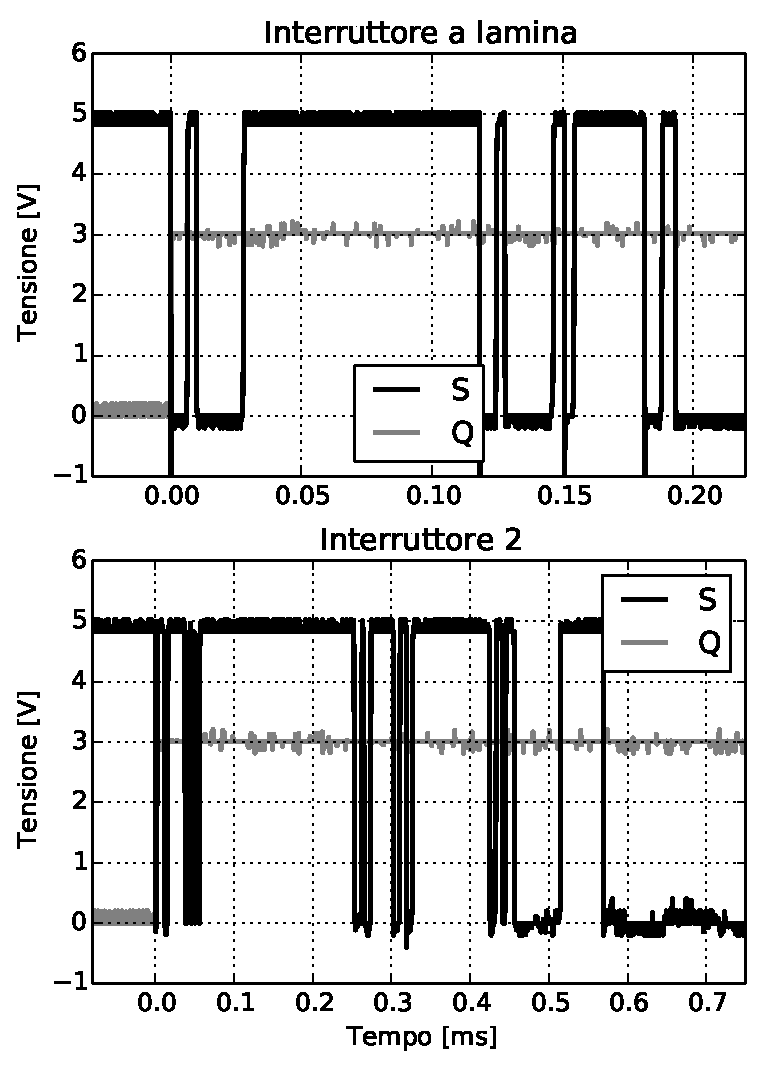
\includegraphics[width=\columnwidth]{figure/rimb.pdf}
	\caption{}
	\label{fig:rimb11}
\end{figure}

Abbiamo provato il circuito con due diversi tipi di interruttori. In un caso abbiamo usato un interruttore a lamina
e un altro interruttore a due stati che dovrebbero generare rumori diversi. La verifica del funzionamento è immediata. Il circuito ha funzionato bene,
cambiando di stato stabilmente senza l'interferenza del rumore. La figura \ref{fig:rimb11} mostra la tensione in S e in Q
per i due interruttori. Come si vede i due interruttori generano molto rumore (S), e il tipo di rumore è diverso tra i due
(quello a lamina dimostra di avere rimbalzi più marcati). Tuttavia l'output è stabile e la commutazione è precisa senza
tracce di rumore. I rimbalzi durano circa 200 $\mu$s.

\paragraph{Divisore di frequenza}

Vediamo ora un applicazione dei flip-flop: il divisore di frequenze. Questo circuito sarebbe molto complesso da
implementare senza flip-flop. Inoltre ha delle applicazioni molto importanti, per esempio i contatori.

\begin{figure}
	\centering
	\begin{circuitikz}
    \draw % primo flip flop
        (-1,-1.6) rectangle (1,1.6)
            (-1,0) ++(0,-0.2) -- ++(0.2,0.2) -- ++(-0.2,0.2)
            (-1,0.8)  node[right] (J1)   {J}
            (-0.8,0)    node[right] (CLK1) {CLK}
            (-1,-0.8) node[right] (K1)   {K}
            (0,-1.6)  node[above] (CL1)  {CL}
            (1,-0.8)  node[left]  (QN1)  {$\overline{\text{Q}}$}
            (1,0.8)   node[left]  (Q1)   {Q}
            (0,1.6)   node[below] (PR1)  {PR}
            % metto i tondini
            (K1.west)   ++(-0.1cm,0cm) circle (0.1cm)
            (PR1.north) ++(0cm,0.1cm)  circle (0.1cm)
            (CL1.south) ++(0cm,-0.1cm) circle (0.1cm)
            % collegamenti
            (J1.west) -- ++(-0.5,0) -- ++(0,0.5) node[above]{$V\ped{CC}$}
            (PR1.north) ++(0cm,0.2cm) -- ++(0,0.5) node[above]{$V\ped{CC}$}
            (CL1.south) ++(0cm,-0.2cm) -- ++(0,-0.5) node[below]{$V\ped{CC}$}
            (K1.west) ++(-0.2cm,0cm) -- ++(-0.8,0) node[rground]{}
        ;
        \draw[xshift=4cm] % secondo flip flop
        (-1,-1.6) rectangle (1,1.6)
            (-1,0) ++(0,-0.2) -- ++(0.2,0.2) -- ++(-0.2,0.2)
            (-1,0.8)  node[right] (J2)   {J}
            (-0.8,0)    node[right] (CLK2) {CLK}
            (-1,-0.8) node[right] (K2)   {K}
            (0,-1.6)  node[above] (CL2)  {CL}
            (1,-0.8)  node[left]  (QN2)  {$\overline{\text{Q2}}$}
            (1,0.8)   node[left]  (Q2)   {Q2}
            (0,1.6)   node[below] (PR2)  {PR}
            % metto i tondini
            (K2.west)   ++(-0.1cm,0cm) circle (0.1cm)
            (PR2.north) ++(0cm,0.1cm)  circle (0.1cm)
            (CL2.south) ++(0cm,-0.1cm) circle (0.1cm)
            % collegamenti
            (J2.west) -- ++(-0.5,0) -- ++(0,0.5) node[above]{$V\ped{CC}$}
            (PR2.north) ++(0cm,0.2cm) -- ++(0,0.5) node[above]{$V\ped{CC}$}
            (CL2.south) ++(0cm,-0.2cm) -- ++(0,-0.5) node[below]{$V\ped{CC}$}
            (K2.west) ++(-0.2cm,0cm) -- ++(-0.8,0) node[rground]{}        
        ;
        % collego i due flip flop e metto le uscite
        \draw
            (Q1.east) -- ++(0.5,0) |- (3, 0)
            (CLK1.west) ++ (-0.2, 0) -- ++(-1,0) node[left]{$V\ped{in}$}
            (Q2.east) -- ++(0.5,0) node[right]{$V\ped{out}$}
        ;
    \end{circuitikz}
	\caption{PR è il preset e CL sta per clear. Entrambi i piedini vanno collegati all'alimentazione
        in modo da non creare problemi.}
	\label{fig:freq_div11}
\end{figure}

\begin{figure}[b]
	\centering
	\begin{circuitikz}
        \draw (0, 0) node[left] {$V\ped{in}$} -| (0.5, 0.5) -| (1, 0) -| (1.5, 0.5) -| (2, 0) -| (2.5, 0.5) -| (3, 0) -| (3.5, 0.5) -| (4, 0);
        \draw (0, -1) node[left] {Q} -| (1, -0.5) -| (2, -1) -| (3, -0.5) -| (4, -1);
    \end{circuitikz}
	\caption{}
	\label{fig:freqs11}
\end{figure}

Il circuito in figura \ref{fig:freq_div11} è un divisore per 4. In questo circuito i rettangoli rappresentano
dei flip-flop di tipo JK, che sono molto simili a quelli di tipo SR. Per costruire il circuito abbiamo usato
l'integrato 74LS109 che contiene 2 FF JK. I flip-flop JK, a differenza di quelli SR, quando sottoposti
all'input $J=1$ e $K=1$ al posto di andare in uno stato indefinito scambiano le uscite Q e $\overline{\text{Q}}$.
In pratica $J=1$ e $K=1$ funziona come un comando di toggle, invertendo lo stato della memoria.
Per il resto si comportano esattamente come gli SR, con J al posto di S e K al posto di R.
Il modello da noi usato è negative edge triggered, ovvero cambia stato quando il clock scende da alto a basso,
mentre negli altri casi l'output rimane costante.

Grazie a questo possiamo vedere che il circuito in figura \ref{fig:freq_div11} funziona nel seguente modo.
Analizziamo solo il primo blocco, poiché il secondo FF è in cascata e serve a dividere ulteriormente per 2 la frequenza.
Inizialmente $V\ped{out} = 0$. Quando giunge un fronte d'onda positivo non succede nulla, poiché il FF è negative edge triggered.
Tuttavia, una volta che
l'input torna a 0 si ha che Q cambia stato salendo a 1 (supponendo che all'inizio fosse nullo).
All'arrivo di un altro
impulso non accade nulla, ma quando arriva la discesa Q cambia stato di nuovo, tornando a 0.
È chiaro che in Q c'è un onda quadra che varia a metà della frequenza del segnale in ingresso.
La figura \ref{fig:freqs11} chiarifica la situazione. 

\begin{figure}
	\centering
	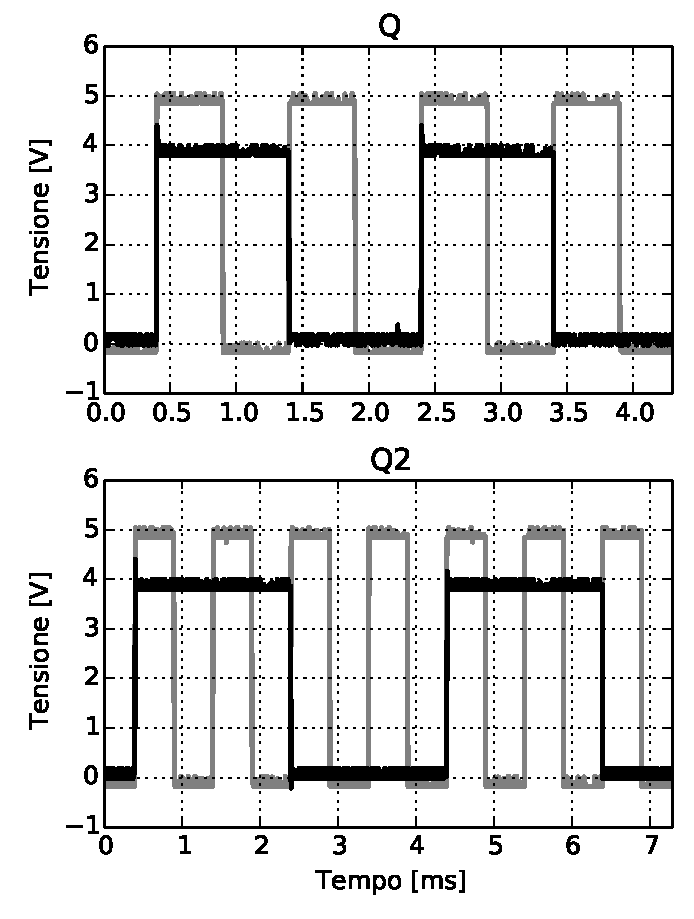
\includegraphics[width=\columnwidth]{figure/freq.pdf}
	\caption{L'input era un onda quadra a 1 kHz.}
	\label{fig:freq_graph11}
\end{figure}

La figura \ref{fig:freq_graph11} mostra invece l'input $V\ped{in}$ (grigio) e i due output del circuito (nero),
mostrando il suo corretto funzionamento.
